\documentclass[12pt]{article}
\usepackage[T1]{fontenc}
\usepackage{graphicx}
\graphicspath{{imagenes/}}

\begin{document}

\begin{flushleft}

\includegraphics[width=2.75cm]{unam.png}\hspace{8cm} 
\includegraphics[width=2.5cm]{fac.png}
\end{flushleft}

\begin{center}
\begin{Huge}
\texttt{UNAM}
\end{Huge}

\vspace{0.5cm}
\begin{LARGE}
\texttt{FACULTAD DE INGENIERIA}

\vspace{0.5cm}
\texttt{INGENIERIA EN COMPUTACION}

\vspace{0.5cm}
\texttt{PROGRAMACION ORIENTADA OBJETOS}

\vspace{0.5cm}
\texttt{ANALISIS PREVIO A LA IMPLEMENTACION}

\vspace{1cm}
\end{LARGE}

\vspace{0.5cm}
\begin{LARGE}
\texttt{CARRILLO SANCHEZ RICARDO\\HERNANDEZ GOMEZ ALEJANDRO\\ZARAZUA RAMIREZ JOHAN AXEL}

\vspace{1cm}
\texttt{GRUPO: 04}

\vspace{1cm}
\texttt{PROFESOR: EDGAR TISTA GARCIA}
\end{LARGE}
\end{center}


\vspace{4cm}
\begin{flushleft}
\begin{Large}
\textbf{Analisi previo a la implementacion de un sistema de administración de hotel}
\end{Large}

\section{Diseño}

\textsf{Para poder hacer el sistema se creo una base de datos con base en el siguiente esquema de entidad relación}

\vspace{0.5cm}
\begin{center}
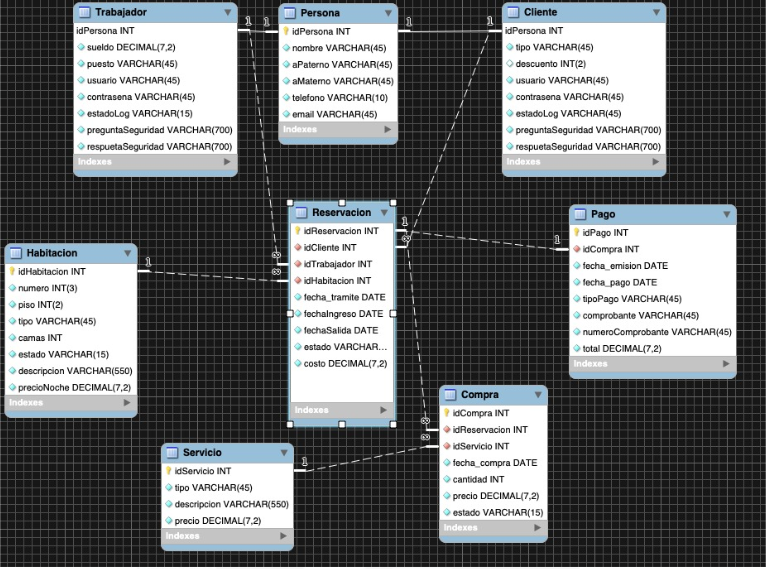
\includegraphics[width=15cm]{EER.png}
\end{center}
\vspace{0.5cm}

\textsf{De esta manera podemos hacer que en una tabla tengamos un columna  con la cual podamos ligar columnas de otra tabla, esto lo hicimos ya que detectamos que en el sistema podríamos tener una composición de objetos ya que una reservación tiene un cliente, un trabajador, una habitación, etc. Por lo tanto pudimos hacer estas composición  a partir de la base datos haciendo que no exista una composición de clases en el código de Java y favoreciendo a una cohesión baja.\\
En cuanto al codigo en java se divide se dividio en 3 paquetes distintos para poder separar nuestras clases y hacernos mas sencilla la solucion de un problema, mantenimiento, etc. En el paquete datos nos encargamos de crear una clase para cada una de las tablas en la base de datos, esto con el fin de almacenar la información necesaria en un objeto y después enviarla a la base de datos mediante este objeto.\\
En el paquete lógico se planeo crear las clases mediante las cuales se haran operaciones en la base de datos como pueden ser consultas, inserciones, actualizaciones o eliminación de datos, en estas clases se penso en las posibles consultas que podríamos hacer por lo cual  podemos ver sobrecarga de metodos en algunas de esta clases.\\
Por ultimo en el paquete visual se crearon cada una de las ventanas que vera el usuario, en ellas el podrá interactuar dependiendo el tipo de usuario que sea.}

\vspace{0.5cm}
\begin{center}
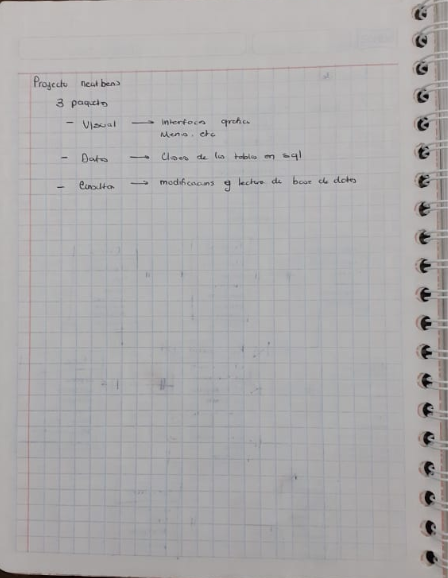
\includegraphics[width=7cm]{diseno1.png}
\end{center}
\vspace{0.5cm}

\vspace{0.5cm}
\begin{center}
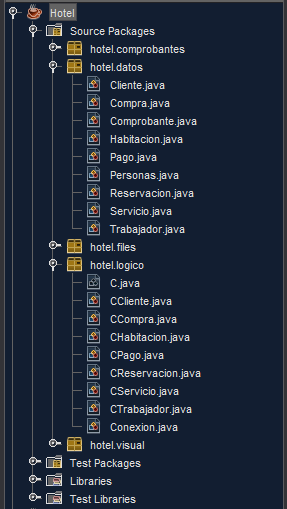
\includegraphics[width=7cm]{diseno2.png}
\end{center}
\vspace{0.5cm}

\textsf{En conclusión podemos decir que las relaciones entre las tablas de la base de datos son muy importantes para el diseño de nuestro problema ya que a partir de ellas podemos hacer que ciertos datos tengan una conexión pero sin depender de otros, por lo que podemos eliminar  sin tanto problema ya que estaremos seguros de que solo se elimina el dato que nos interesa y no otros datos, esto lo podemos ver en la relación de pagos y reservación ya que podemos eliminar un pago sin eliminar una reservación, en cambio si esto se realiza por composicion de objetos podría darse el caso de que al eliminar un pago también eliminemos una reservación,  si esto lo vemos en un aspecto Real podría suceder que un trabajador se equivoque al registrar un pago y al eliminarlo, eliminaría con el a la reservación por lo que tendrías que volver a crear la reservación y posteriormente crear de nuevo el pago}


\end{flushleft}
\end{document}
